
%%%%%%%%%%%%%%%%%%%%%%%%%%%%%%%%%%%%%%%%%%%%%%%%%%%%%%%%%%%%%%%
%
% Welcome to Overleaf --- just edit your LaTeX on the left,
% and we'll compile it for you on the right. If you open the
% 'Share' menu, you can invite other users to edit at the same
% time. See www.overleaf.com/learn for more info. Enjoy!
%
%%%%%%%%%%%%%%%%%%%%%%%%%%%%%%%%%%%%%%%%%%%%%%%%%%%%%%%%%%%%%%%
\documentclass{beamer}
\usepackage{braket}
\usepackage{amssymb}

%Information to be included in the title page:
\title{HHL - Algorithmus}
\author{Alfred Nguyen}
\institute{Fakultät der Informatik \\
Technische Universität München \\
  85758 Garching, Bavaria
}
\date{June 2023}

\setbeamertemplate{navigation symbols}{}
\setbeamertemplate{footline}[frame number]

\AtBeginSection[]
{
  \begin{frame}
    \frametitle{Gliederung}
    \tableofcontents[currentsection]
  \end{frame}
}

\begin{document}

  \frame{\titlepage}
  \begin{frame}
    \frametitle{Gliederung}
    \tableofcontents
  \end{frame}
  
%\section{Einführung}

%\subsubsection{Quanten Algorithmen}

    \begin{frame}
        \frametitle{Einführung}
        Wir haben schon viel über die wichtigsten Algorithmen gehört
        \begin{itemize} 
            \item  Shors-Algorithmus
            \item  Grover-Algorithmus
        \end{itemize}

        \hfill

\onslide<2>{
        Der HHL-Algorithmus
        \begin{itemize}
            \item  erstellt von Aram Harrow, Avinatan Hassidim und Seth Lloyd 
            \item  lösen von sehr großen linearen Gleichungen 
        \end{itemize}

        $$ A \vec{x} = \vec{b} $$
}

    \end{frame}


%\subsubsection{Motivation}

    \begin{frame}
        \frametitle{Motivation}

        Es löst grundlegendes Probleme in der Mathematik
        \begin{itemize}
            \item   Least square fitting 
            \item   Optimierungs Probleme
            \item   Simulationen und Imageprocessing
            \item   ...
       \end{itemize}

        \hfil

    \end{frame}

%\subsubsection{Das Problem}
    \begin{frame}
        \frametitle{Das Problem}


        \textbf{Gegeben:}
        \begin{itemize}
            \item Matrix $A$ der Form $n \times n$
            \item Vektor $\vec{b}$
       \end{itemize}

       \hfill

\onslide<2,3>{
       \textbf{Löse das System:}
        $$A \vec{x} = \vec{b}$$

        $$\vec{x} = A^{-1} \vec{b}$$
}
       \hfill

\onslide<3>{

        Wir sind also daran interessiert das Inverse $A^{-1}$ zu finden
}

    \end{frame}
        


%\section{Mathematische Grundlagen}

\begin{frame}
    \frametitle{Hermitsche Matrix}
    \textbf{Sei: }
    \begin{itemize}
        \item   $A$ eine $n \times n$ Matrix
        \item   $A^T$ das transponierte von $A$
        \item   $\overline A$  das komplex konjugierter von $A$
        \item   $A^\dagger$ die Hermitsche Matrix von A
   \end{itemize}

   \hfil

    \textbf{Dann:}
    $$A = \overline {A^T} = A^\dagger $$
\end{frame}

\begin{frame}
    \frametitle{Hermitsche Matrix}
    
    \textbf{Beispiel:}
    $$A=\begin{bmatrix}2 & 1-i \\ 1+i & 3 \\ \end{bmatrix}$$
    $$\overline A = \begin{bmatrix} 2 & 1+i \\ 1-i & 3 \end{bmatrix}$$
    $$\overline {A^T} = \begin{bmatrix} 2 & 1-i \\ 1+i & 3 \\ \end{bmatrix}= A = A^\dagger$$

    \hfil

    \hfil

    Die Matrix $A$ ist Hermitisch.
\end{frame}

\begin{frame}
    \frametitle{Hermitsche Matrix}
    
    Falls eines Matrix $A$ nicht Hermitisch ist:

    \hfil

    $$A^\dagger = \begin{pmatrix} 0 & A \\ \overline {A^T} & 0 \end{pmatrix}$$
\end{frame}


\begin{frame}
    \frametitle{Spektralzerlegung}

    \textbf{Gegeben: }

    $$A =  U D U^T$$

    $$= \begin{bmatrix} U_1&U_2&...&U_n \end{bmatrix}
    \begin{bmatrix} \lambda_1 & 0 & 0 & 0\\ 0 & \lambda_2 &0 & 0\\ 0 & 0 & ... & 0\\ 0 & 0 & 0& \lambda_n \\ \end{bmatrix}
    \begin{bmatrix} U_1\\ U_2\\ ...\\ U_n\end{bmatrix}$$

    \hfil

    \begin{itemize}
        \item   $A$ eine $n \times n$ Matrix
        \item   $D$ ist eine Diagonalmatrix aus den Eigenwerten
        \item   $U$ besteht aus den Eigenvektoren von A
   \end{itemize}



    \hfil

    $A$ lässt sich aus seinen Eigenweren und Eigenvektoren darstellen.

\end{frame}

\begin{frame}
    \frametitle{Spektralzerlegung}
    Selbes gilt für das Inverse von $A$ 

    $$A^{-1}=  U^T D^{-1} U$$

    \hfil

    \begin{itemize}
        \item  $A^{-1}$ nur durch Eigenwerten und Eigenvektoren bestimmbar!
        \item  Methode im klassischen nicht schneller
        \item  für HHL Algorithmus sehr wichtig
   \end{itemize}
\end{frame}

\begin{frame}
    \frametitle{Veschränkung}
    
    Verschränkte Zustände können nicht durch einzelne Zustände dargestellt werden

    \hfil

    $$\ket{\Phi} \neq \ket{\phi} \ket{\psi}$$

\end{frame}

\begin{frame}
    \frametitle{Veschränkung}
    \textbf{Beispiel:}

    \hfil

    \begin{columns}[c]
        \begin{column}{0.6\hsize}\centering
        Nicht Verschränkt
        $$\ket{\Phi_1} = \frac{1}{\sqrt{2}} ( \ket{10} + \ket{11})$$
        $$= \ket{1}\otimes \frac{1}{\sqrt{2}} ( \ket{0} + \ket{1})= \ket{1} \ket{+}$$
        \end{column}

        \begin{column}{0.4\hsize}
        Verschränkt
        $$\ket{\Phi_2} = \frac{1}{\sqrt{2}} ( \ket{00} + \ket{11})$$
        $$\neq \ket{\alpha}\ket{\beta}$$

        \end{column}
    \end{columns}

\end{frame}

\section{HHL Algorithmus}

%\subsubsection{Übersicht}

    \begin{frame}
    \frametitle{Übersicht}
    Vergleich klassische zur quanten Version

    \hfil

    \begin{columns}[c]
        \begin{column}{0.6\hsize}\centering
        Klassisch
        $$A \vec{x} = \vec{b}$$
        $$\vec{x} = A^{-1}\vec{b}$$
        \end{column}

        \begin{column}{0.4\hsize}
        Quanten Version
        $$A \ket{x} = \ket{b}$$
        $$\ket{x} = A^{-1}\ket{b}$$
        \end{column}
    \end{columns}

    \hfil

    \hfil
    
    Spektralzerlegung von $A$ und $\ket{b}$
    $$\ket{x} =  A^{-1} \ket{b} = \sum_{i=0}^{2^{n_b}-1} \lambda_i^{-1} b_j\ket{u_j}$$

    \end{frame}


%\subsubsection{Der Algorithmus}

    \begin{frame}
    \frametitle{Der Algorithmus}

        \textbf{Ablauf}
        \begin{enumerate}
            \item State Preparation
            \begin{itemize}
                \item Enkodiert Vektor und Matrix in Quanten Computer
            \end{itemize}
            \item Quantum Phase Estimation
            \begin{itemize}
                \item ermittelt Eigenwerte 
            \end{itemize}
            \item Ancilla Bit Rotation 
            \begin{itemize}
                \item  Invertiert Eigenwerte
            \end{itemize}
            \item Inverse Quantum Phase Estimation
             \begin{itemize}
                \item löst verschränkte Qubits auf
            \end{itemize}
            
            \item Messung
             \begin{itemize}
                \item liest das Ergebnis $\ket{x}$ aus
            \end{itemize}
 
        \end{enumerate}

    \end{frame}

\begin{frame}
    \frametitle{Quantum Circuit}
    \begin{center}
    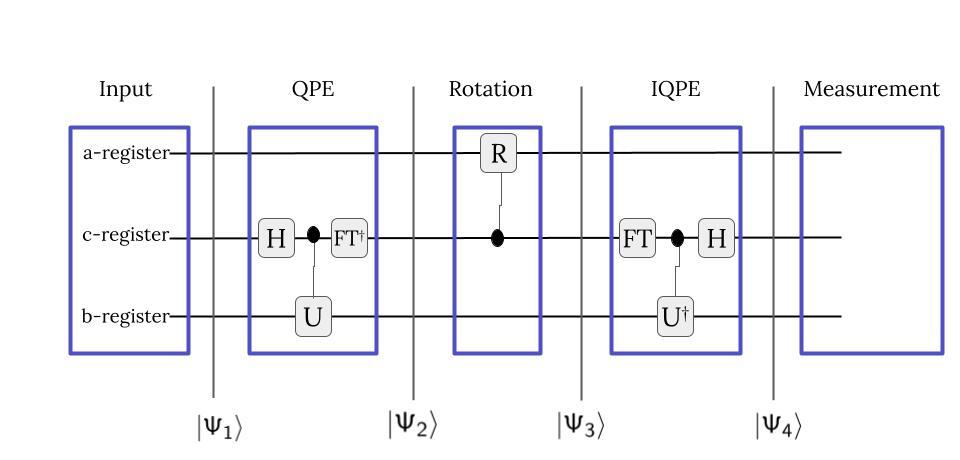
\includegraphics[width=10.5cm]{img/hhl_circuit/hhl_circuit.jpg}
    \end{center}
    \begin{enumerate}
        \item Ancilla (Helfer): a-register
        \begin{itemize}
            \item Indikator qubit, zeigt ob Zustände verschränkt sind
        \end{itemize}

        \item Register: c-register
        \begin{itemize}
            \item beinhaltet die Eigenwerte
        \end{itemize}
        
        \item Input: b-register 
        \begin{itemize}
            \item beinhaltet den Vektor $\vec{b}$
        \end{itemize}
        
    \end{enumerate}
   \end{frame}


    \begin{frame}
    \frametitle{Was das}

        \textbf{Ablauf}
        \begin{enumerate}
            \item State Preparation
            \begin{itemize}
                \item Enkodiere Vektor und Matrix in Quanten Computer
            \end{itemize}
            \item Quantum Phase Estimation
            \begin{itemize}
                \item ermittle Eigenwerte und Eigenvektoren 
                \item bilde $\ket{b}$ in Eigenbasis $A$ ab
            \end{itemize}
 
            \item Ancilla Bit Rotation - Invertieren der Eigenwerte
            \item Inverse Quantum Phase Estimation
            \item Messung

        \end{enumerate}
 
    

    \end{frame}


\end{document}